\documentclass[aspectratio=169,11pt,xcolor=table]{beamer}

\usepackage[utf8]{inputenc}
% Portable: usa babel español y Latin Modern si están instalados (Overleaf los tiene)
\IfFileExists{spanish.ldf}{\usepackage[spanish,es-nodecimaldot,es-noshorthands]{babel}}{}
\IfFileExists{lmodern.sty}{\usepackage[T1]{fontenc}\usepackage{lmodern}}{}
\usepackage{amsmath,amssymb}
\usepackage{booktabs}
\usepackage{array}
\usepackage{tabularx}
\newcolumntype{L}[1]{>{\raggedright\arraybackslash}p{#1}}
\newcolumntype{Y}{>{\raggedright\arraybackslash}X}
% Imagen a pantalla completa (debajo del título)
\newcommand{\fullfig}[1]{\vspace{-0.15cm}\begin{center}\makebox[\textwidth]{\includegraphics[width=0.97\paperwidth,height=0.76\textheight,keepaspectratio]{#1}}\end{center}\vspace{-0.2cm}}
\usepackage{graphicx}
\usepackage{appendixnumberbeamer}
\usepackage{tikz}
\usetikzlibrary{positioning,arrows.meta,decorations.pathreplacing}

% ---------------- Estilo ----------------
\definecolor{upblue}{HTML}{1E3A8A}
\definecolor{upaccent}{HTML}{2E6FD8}
\definecolor{upgray}{HTML}{5B6170}
\definecolor{upred}{HTML}{C0392B}
\definecolor{uplight}{HTML}{EEF2FA}

\usetheme{default}
\setbeamertemplate{navigation symbols}{}
\setbeamercolor{frametitle}{fg=upblue}
\setbeamerfont{frametitle}{series=\bfseries,size=\Large}
\setbeamercolor{structure}{fg=upblue}
\setbeamercolor{normal text}{fg=black!85}
\setbeamercolor{alerted text}{fg=upred}
\setbeamertemplate{itemize items}{\color{upaccent}$\blacktriangleright$}
\setbeamertemplate{itemize subitem}{\color{upgray}--}
% Más espacio entre bullets
\newcommand{\itemgap}{1.3em}
\makeatletter
\let\OLDitemize\itemize
\renewcommand\itemize{\OLDitemize\ifnum\@itemdepth=1\setlength{\itemsep}{\itemgap}\else\setlength{\itemsep}{0.4em}\setlength{\topsep}{0.5em}\fi}
\makeatother
\setbeamercolor{block title}{bg=upblue,fg=white}
\setbeamercolor{block body}{bg=uplight}
\setbeamertemplate{blocks}[rounded][shadow=false]

\setbeamertemplate{frametitle}{%
  \vspace{0.35cm}\insertframetitle\par
  \vspace{-0.1cm}{\color{upaccent}\rule{2.2cm}{1.5pt}}%
}
\setbeamertemplate{footline}{%
  \hbox{\begin{beamercolorbox}[wd=\paperwidth,ht=3ex,dp=1.2ex]{}%
    
    \hfill{\color{upgray}\tiny\insertframenumber/\inserttotalframenumber}\hspace{0.4cm}%
  \end{beamercolorbox}}%
}

\newcommand{\hl}[1]{\textcolor{upaccent}{\textbf{#1}}}
% Celda de N.° de distritos: reemplazar \dist{} por \dist{1\,828}, etc.
\newcommand{\dist}[1]{\textcolor{upaccent}{\if\relax\detokenize{#1}\relax\textit{\small por completar}\else\textbf{#1}\fi}}

% ---------------- Portada ----------------
\title{Voto obligatorio, envejecimiento y la brecha de participación a los 70 años}
\subtitle{Un modelo para datos electorales por grupo etario}
\author{Manuel Alfredo Arriola Montenegro}
\institute{Inteligencia Artificial y Modelamiento Económico, Universidad del Pacífico}
\date{7 de octubre de 2026}

\begin{document}

% ===== 1. Portada (0:30) =====
{
\setbeamertemplate{footline}{}
\begin{frame}
  \begin{center}
    
\includegraphics[height=1.4cm]{logo.png}\\[0.6cm]
    {\color{upblue}\Large\bfseries \inserttitle}\\[0.2cm]
    {\color{upgray}\large \insertsubtitle}\\[0.7cm]
    {\small \textbf{Manuel Alfredo Arriola Montenegro}}\\[0.25cm]
    {\small Topic presentation \;\textbar\; Track B: modelo de tesis}\\[0.15cm]
    {\footnotesize\color{upgray} Inteligencia Artificial y Modelamiento Económico \;\textbar\; Lima, 7 de octubre de 2026}\\[0.25cm]
    {\small\color{upaccent}\href{https://github.com/Arriola123456/ai-project}{\texttt{github.com/Arriola123456/ai-project}}}
  \end{center}
\end{frame}
}

% ===== 2. Motivación (1:00) =====
\begin{frame}[c]{Motivación: la participación cae a los 70}
  \fullfig{grafico1.png}
  {\centering\tiny Participación = sufragantes / habilitados (no omisos). Fuente: ONPE. Elaboración propia.\par}
\end{frame}

% ===== 3. Pregunta (1:00) =====
\begin{frame}{La pregunta de la tesis y el problema del modelo}
  \begin{block}{Pregunta de la tesis}
    ¿Cuál es la \textbf{magnitud} y la \textbf{estabilidad} de la brecha de participación entre 60-69 y 70+, y \textbf{varía con la multa} por omisión?
  \end{block}
  \vspace{0.3cm}
  \begin{itemize}
    \item ONPE reporta la edad en \hl{intervalos} y el grupo 70+ es \hl{abierto}.
    \item La brecha mezcla el \textbf{fin de la obligatoriedad} con el \textbf{envejecimiento}.
    \item El modelo de la tesis describe a un votante \textit{individual}, pero los datos son \textit{agregados}.
  \end{itemize}
  \vspace{0.2cm}
  \begin{block}{}
    \centering El modelo debe decir \textbf{qué mide la brecha observada}.
  \end{block}
\end{frame}

% ===== 4. Hoja de ruta (0:45) =====
\begin{frame}{Qué propongo en este curso}
  \begin{columns}[T]
    \begin{column}{0.32\textwidth}\centering
      {\color{upaccent}\Large\bfseries Modelo}\\[0.15cm]\small Cálculo del voto con obligatoriedad (Panagopoulos, 2008), extendido con perfil por edad y hábito.
    \end{column}
    \begin{column}{0.32\textwidth}\centering
      {\color{upaccent}\Large\bfseries Supuesto}\\[0.15cm]\small Relajo que se observe la participación \textbf{individual}: solo se observan tasas por \textbf{grupo etario}.
    \end{column}
    \begin{column}{0.32\textwidth}\centering
      {\color{upaccent}\Large\bfseries Resultado}\\[0.15cm]\small Caracterizar el efecto causal $\tau^{70}$ y la \textbf{brecha agregada} $\Delta$, y su respuesta a la multa, la edad y la heterogeneidad.
    \end{column}
  \end{columns}
\end{frame}

% ===== 4b. Downs (1:00) =====
\begin{frame}{Literatura (1/4): Downs (1957)}
  \begin{block}{Regla de decisión}
    \[ \text{vota} \iff R = p\,B - C > 0 \]
  \end{block}
  \vspace{0.2cm}
  \begin{itemize}
    \item $p$: probabilidad de que el voto sea \hl{decisivo}; $B$: beneficio diferencial de que gane el candidato preferido; $C$: costo de votar.
    \item Primera formulación del voto como decisión \textbf{costo-beneficio}.
    \item \alert{Paradoja del voto}: en electorados grandes $p\approx 0$, así que nadie debería votar.
  \end{itemize}
\end{frame}

% ===== 4c. Riker y Ordeshook (1:00) =====
\begin{frame}{Literatura (2/4): Riker y Ordeshook (1968)}
  \begin{block}{Regla de decisión}
    \[ \text{vota} \iff R = p\,B - C + D > 0 \]
  \end{block}
  \vspace{0.2cm}
  \begin{itemize}
    \item $D$: beneficio del \hl{acto mismo de votar} (deber cívico, expresión, afirmar la democracia).
    \item Resuelve la paradoja: aun con $p\approx 0$, se vota si $D>C$.
    \item Tanto votar como abstenerse pueden ser decisiones \textbf{racionales}.
  \end{itemize}
\end{frame}

% ===== 4d. Panagopoulos (1:00) =====
\begin{frame}{Literatura (3/4): Panagopoulos (2008)}
  \begin{block}{Regla de decisión con voto obligatorio}
    \[ \text{vota} \iff p\,B - C + D + S > 0 \]
  \end{block}
  \vspace{0.2cm}
  \begin{itemize}
    \item $S$: \hl{costo esperado de abstenerse}, la multa ponderada por la probabilidad de que se cobre.
    \item La obligatoriedad no cambia el beneficio de votar: \textbf{encarece no votar}.
    \item Su peso depende del monto de la sanción y de su aplicación efectiva (Blais, 2006).
  \end{itemize}
  \vspace{0.1cm}
  {\scriptsize\color{upgray} Notación adaptada para comparar con los modelos anteriores.\par}
\end{frame}

% ===== 4e. Fowler (1:00) =====
\begin{frame}{Literatura (4/4): J.\,H.\ Fowler (2006)}
  \begin{block}{Propensión a votar con aprendizaje adaptativo}
    \[ \pi_{i,t+1}=\begin{cases} \pi_{it}+\eta\,(1-\pi_{it}) & \text{si la acción tomada en } t \text{ satisfizo la aspiración}\\[0.1cm] \pi_{it}-\eta\,\pi_{it} & \text{si no la satisfizo}\end{cases} \]
  \end{block}
  \vspace{0.1cm}
  \begin{itemize}
    \item $\pi_{it}$: propensión a votar; $\eta$: velocidad de aprendizaje. Las acciones satisfactorias se \hl{refuerzan}.
    \item La participación pasada eleva la futura: \textbf{hábito} y patrones estables de voto u omisión.
    \item En mi modelo lo simplifico como un stock $h$ que eleva el beneficio de votar.
  \end{itemize}
  \vspace{0.05cm}
  {\scriptsize\color{upgray} Esquema de refuerzo, notación adaptada; la regla aplica a la acción elegida (votar o abstenerse).\par}
\end{frame}

% ===== 5. Modelo base y supuestos relajados (1:30) =====
\begin{frame}{Modelo base y supuestos que relajo}
  \small Base: \textbf{Riker y Ordeshook (1968); Panagopoulos (2008)}. Se vota si el beneficio neto de votar supera el costo de abstenerse, que incluye la sanción esperada.
  \vspace{0.25cm}

  \renewcommand{\arraystretch}{1.45}
  \begin{tabularx}{\textwidth}{@{}L{1.0cm}L{4.3cm}Y@{}}
    \toprule
    & \textbf{Supuesto del modelo base} & \textbf{Relajación} \\
    \midrule
    (S1) & Beneficio invariante a la edad & El beneficio de votar sigue un ciclo de vida y cae en edades avanzadas (Bhatti et al., 2012) \\
    \rowcolor{uplight}(S2) & Se observa la participación individual & Solo tasas por \textbf{grupo etario}; 70+ abierto. \hl{Genera el resultado.} \\
    (S3) & Sin persistencia & Votar acumula \textbf{hábito} (J.\,H.\ Fowler, 2006), mecanismo complementario \\
    \bottomrule
  \end{tabularx}
\end{frame}

% ===== 6. Modelo: utilidad (1:30) =====
\begin{frame}{Modelo: utilidad dada la obligación}
  \small
  \renewcommand{\itemgap}{0.45em}
  \begin{itemize}
    \item $B(a,h)$: \hl{beneficio neto de votar}, depende de la edad $a$ y del hábito $h$.
    \item $c$: \hl{costo individual de votar}, heterogéneo, con distribución $G$ y densidad $g$.
    \item $O=\mathbf{1}[a<70]$: indicador de \hl{obligación}; $S=qF$: sanción esperada por abstenerse.
  \end{itemize}
  \vspace{0.1cm}
  \begin{block}{Utilidad de cada alternativa}
    \[ U(v=1)=B(a,h)-c, \qquad U(v=0)=-\,O\,S \]
  \end{block}
  \vspace{0.05cm}
  \begin{block}{Probabilidad de votar, con y sin obligación}
    \vspace{-0.15cm}
    \begin{align*}
      P_1(a) &\equiv \Pr\big[v=1 \mid O=1\big]=\Pr\big[B(a,h)-c>-S\big] \\
      P_0(a) &\equiv \Pr\big[v=1 \mid O=0\big]=\Pr\big[B(a,h)-c>0\big]
    \end{align*}
  \end{block}
\end{frame}

% ===== 6a. Decisión de cada individuo (1:00) =====
\begin{frame}{¿Cuándo vota cada individuo?}
  \begin{columns}[T]
    \begin{column}{0.48\textwidth}
      \begin{block}{Obligado ($a<70$, $O=1$)}
        \small Vota sí si
        \[ B(a,h)-c>-S \iff c<B(a,h)+S \]
        \vspace{-0.3cm}
        \[ \Rightarrow\quad P_1(a)=G\big(B(a,h)+S\big) \]
      \end{block}
    \end{column}
    \begin{column}{0.48\textwidth}
      \begin{block}{No obligado ($a\ge 70$, $O=0$)}
        \small Vota sí si
        \[ B(a,h)-c>0 \iff c<B(a,h) \]
        \vspace{-0.3cm}
        \[ \Rightarrow\quad P_0(a)=G\big(B(a,h)\big) \]
      \end{block}
    \end{column}
  \end{columns}
  \vspace{0.35cm}
  \begin{block}{Condición de corte del votante marginal (análogo de la CPO)}
    \[ v=1 \iff c< c^*(a)\equiv B(a,h)+O\,S \]
  \end{block}
  {\scriptsize\color{upgray} La decisión es discreta: no hay óptimo interior. El margen relevante es el costo que deja indiferente al ciudadano.\par}
\end{frame}

% ===== 6c. De 70- a 70+ (1:30) =====
\begin{frame}{De $70^-$ a $70^+$: cambio en la probabilidad de votar}
  \small Si $B$ es continuo en la edad, en el umbral solo cambia la obligación:
  \begin{block}{Efecto causal de la obligatoriedad}
    \[ \tau^{70}\equiv\lim_{a\uparrow 70}P_1(a)-\lim_{a\downarrow 70}P_0(a)=G\big(B(70,h)+S\big)-G\big(B(70,h)\big)=\int_{B(70,h)}^{B(70,h)+S} g(c)\,dc>0 \]
  \end{block}
  \vspace{0.15cm}
  \renewcommand{\itemgap}{0.6em}
  \begin{itemize}
    \item $\tau^{70}$ es la masa de \hl{\textit{compliers}}: ciudadanos con costo en la banda $\big[B(70,h),\,B(70,h)+S\big)$, que votan solo porque están obligados.
    \item Quien tiene $c<B(70,h)$ vota en ambos regímenes; quien tiene $c\ge B(70,h)+S$ no vota en ninguno.
    \item El ancho de la banda es $S$; su masa depende de \textbf{dónde} cae en la distribución de costos.
  \end{itemize}
\end{frame}

% ===== 6b. Línea de tiempo (1:30) =====
\begin{frame}[c]{Seguimos a un mismo individuo $i$ en cada elección $t$}
  \centering
  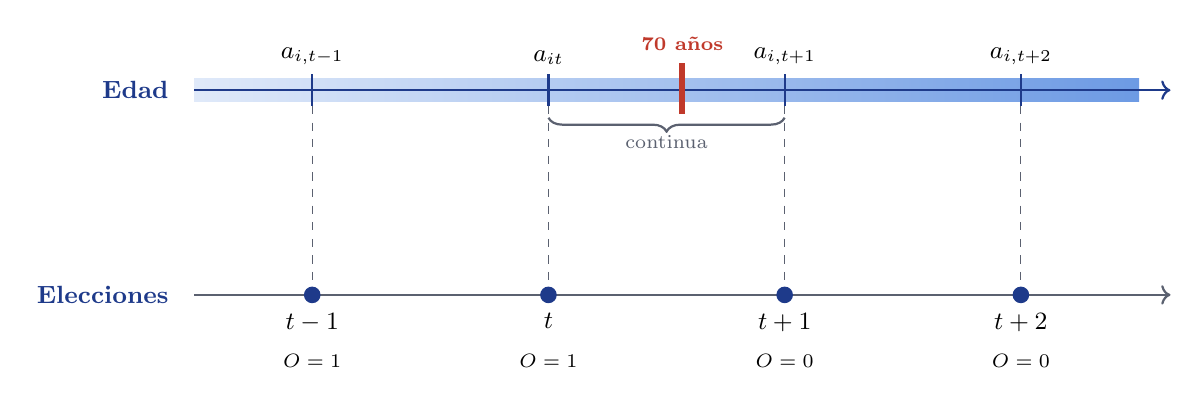
\begin{tikzpicture}[x=1cm,y=1cm]
    % --- linea superior: edad continua ---
    \node[font=\small\bfseries,upblue,anchor=east] at (-0.2,2.6) {Edad};
    \fill[left color=upaccent!15,right color=upaccent!70] (0,2.45) rectangle (12,2.75);
    \draw[->,thick,upblue] (0,2.6) -- (12.4,2.6);
    \foreach \x/\l in {1.5/{a_{i,t-1}},4.5/{a_{it}},7.5/{a_{i,t+1}},10.5/{a_{i,t+2}}}{
      \draw[thick,upblue] (\x,2.4) -- (\x,2.8);
      \node[font=\small,above] at (\x,2.8) {$\l$};
    }
    % umbral 70
    \draw[line width=2.2pt,upred] (6.2,2.3) -- (6.2,2.95) node[above,font=\scriptsize\bfseries]{70 años};
    % llave entre a_t y a_t+1
    \draw[decorate,decoration={brace,amplitude=5pt,mirror},thick,upgray] (4.5,2.25) -- (7.5,2.25) node[midway,below=5pt,font=\scriptsize,upgray,fill=white,inner sep=1pt]{continua};
    % conectores
    \foreach \x in {1.5,4.5,7.5,10.5}{\draw[dashed,upgray] (\x,2.4) -- (\x,0.15);}
    % --- linea inferior: elecciones discretas ---
    \node[font=\small\bfseries,upblue,anchor=east] at (-0.2,0) {Elecciones};
    \draw[->,thick,upgray] (0,0) -- (12.4,0);
    \foreach \x/\l/\o in {1.5/{t-1}/1,4.5/{t}/1,7.5/{t+1}/0,10.5/{t+2}/0}{
      \fill[upblue] (\x,0) circle (3pt);
      \node[font=\small,below=3pt] at (\x,0) {$\l$};
      \node[font=\scriptsize,below=18pt] at (\x,0) {$O=\o$};
    }
  \end{tikzpicture}\\[0.4cm]
  \small
  $a_{i,t+1}=a_{it}+d_t\neq a_{it}$, con $d_t$ los años entre elecciones. La decisión $v_{it}$ solo se toma en cada $t$, pero la edad, y con ella $B(a,h)$ y $O$, cambia entre elecciones.\\[0.15cm]
  {\scriptsize\color{upgray} El hábito también se mueve entre elecciones: $h_{i,t+1}$ depende de $h_{it}$ y de $v_{it}$.\par}
\end{frame}

% ===== 7. Del individuo al grupo (1:30) =====
\begin{frame}{Del votante individual a la brecha por grupos}
  \small
  Con el hábito igual entre ciudadanos ($h=\bar h$), los datos por grupo etario promedian $P_1$ y $P_0$ dentro de cada intervalo:
  \begin{columns}[T]
    \begin{column}{0.48\textwidth}
      \begin{block}{Efecto causal en el umbral}
        \footnotesize
        \[ \tau^{70}=P_1(70)-P_0(70) \]
        Compara al mismo ciudadano a los 70, con y sin obligación. No es observable con datos por intervalos.
      \end{block}
    \end{column}
    \begin{column}{0.48\textwidth}
      \begin{block}{Lo que identifican los datos por grupo}
        \footnotesize
        \[ \Delta=\mathbb E_{a\in[60,70)}\big[P_1(a)\big]-\mathbb E_{a\ge 70}\big[P_0(a)\big] \]
        Esperanzas sobre las edades dentro de cada grupo.
      \end{block}
    \end{column}
  \end{columns}
\end{frame}

% ===== 8. Esquema (1:00) =====
\begin{frame}[c]{Dos caídas superpuestas: $\Delta$ no es $\tau^{70}$}
  \centering
  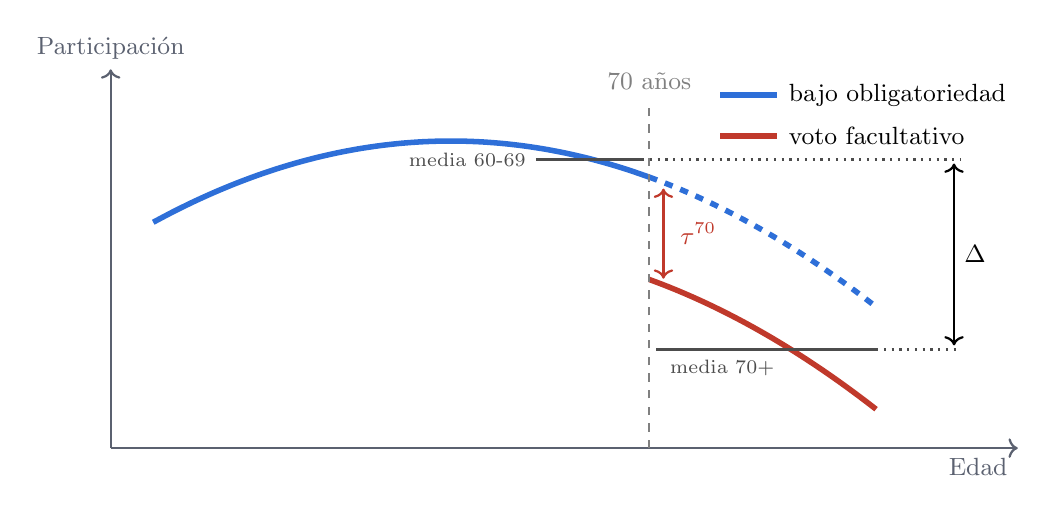
\begin{tikzpicture}[xscale=1.8,yscale=1.3]
    \draw[->,thick,upgray] (0,0) -- (6.4,0) node[below left,font=\small]{Edad};
    \draw[->,thick,upgray] (0,0) -- (0,3.7) node[above,font=\small]{Participación};
    \draw[line width=2pt,upaccent,domain=0.3:3.8,smooth] plot (\x,{3-0.18*(\x-2.4)^2});
    \draw[line width=2pt,upaccent,dashed,domain=3.8:5.4,smooth] plot (\x,{3-0.18*(\x-2.4)^2});
    \draw[line width=2pt,upred,domain=3.8:5.4,smooth] plot (\x,{2.0-0.18*(\x-2.4)^2});
    \draw[dashed,gray,thick] (3.8,0) -- (3.8,3.4) node[above,font=\small]{70 años};
    \draw[<->,thick,upred] (3.9,{3-0.18*(3.9-2.4)^2-0.06}) -- (3.9,{2.0-0.18*(3.9-2.4)^2+0.06});
    \node[font=\small,upred,right] at (3.95,{2.5-0.18*(3.9-2.4)^2}) {$\tau^{70}$};
    % promedios por grupo
    \draw[thick,black!70] (3.0,{3-0.18*(3.4-2.4)^2}) -- (3.75,{3-0.18*(3.4-2.4)^2}) node[left,pos=0,font=\scriptsize]{media 60-69};
    \draw[thick,black!70] (3.85,{2.0-0.18*(4.8-2.4)^2}) -- (5.4,{2.0-0.18*(4.8-2.4)^2}) node[pos=0.3,below,font=\scriptsize]{media 70+};
    \draw[dotted,thick,black!70] (3.75,{3-0.18*(3.4-2.4)^2}) -- (6.0,{3-0.18*(3.4-2.4)^2});
    \draw[dotted,thick,black!70] (5.4,{2.0-0.18*(4.8-2.4)^2}) -- (6.0,{2.0-0.18*(4.8-2.4)^2});
    \draw[<->,thick,black] (5.95,{3-0.18*(3.4-2.4)^2-0.04}) -- (5.95,{2.0-0.18*(4.8-2.4)^2+0.04}) node[midway,right,font=\small]{$\Delta$};
    % leyenda
    \draw[line width=2pt,upaccent] (4.3,3.45) -- (4.7,3.45) node[right,font=\small,black]{bajo obligatoriedad};
    \draw[line width=2pt,upred] (4.3,3.05) -- (4.7,3.05) node[right,font=\small,black]{voto facultativo};
  \end{tikzpicture}\\[0.2cm]
  {\scriptsize\color{upgray} Esquema ilustrativo. La brecha entre medias de grupo suma el salto en el umbral y la caída por edad dentro de cada intervalo.}
\end{frame}

% ===== 8b. Resultados esperados sobre tau (2:00) =====
\begin{frame}{Resultados esperados (1/3): el efecto causal $\tau^{70}$}
  \footnotesize Con $c_0\equiv B(70,h)$ y $c_1\equiv B(70,h)+S$, los extremos de la banda de \textit{compliers}:
  \vspace{0.1cm}
  \begin{columns}[T]
    \begin{column}{0.48\textwidth}
      \begin{block}{(a) Sanción}
        \[ \frac{\partial\tau^{70}}{\partial S}=g(c_1)>0 \]
        \footnotesize Más multa suma a los votantes marginales en $c_1$.
      \end{block}
      \vspace{0.1cm}
      \begin{block}{(b) Curvatura}
        \[ \frac{\partial^2\tau^{70}}{\partial S^2}=g'(c_1)<0 \]
        \footnotesize Si $c_1$ está por encima de la moda de los costos.
      \end{block}
    \end{column}
    \begin{column}{0.48\textwidth}
      \begin{block}{(c) Beneficio a los 70}
        \[ \frac{\partial\tau^{70}}{\partial B(70,h)}=g(c_1)-g(c_0) \]
        \footnotesize Signo ambiguo: si la banda está por encima de la moda, un menor beneficio a los 70 \textbf{amplía} $\tau^{70}$.
      \end{block}
      \vspace{0.1cm}
      \begin{block}{(d) Heterogeneidad}
        \[ \frac{\partial\tau^{70}}{\partial s}<0 \]
        \footnotesize Si $G$ tiene dispersión $s$ y densidad simétrica, y $P_0(70)\le 50\%<P_1(70)$.
      \end{block}
    \end{column}
  \end{columns}
\end{frame}

% ===== 9. Resultados esperados (i)-(ii) (2:00) =====
\begin{frame}{Resultados esperados (2/3): la brecha observada $\Delta$}
  \small Supuesto: el beneficio $B$ no crece con la edad desde los 60 años.
  \vspace{0.2cm}
  \begin{block}{(i) Sesgo por envejecimiento}
    \[ \Delta\ \ge\ \tau^{70}>0 \]
    \footnotesize La brecha observada es una \textbf{cota superior} del efecto de la obligatoriedad: suma el salto en el umbral y la caída por edad dentro de cada grupo.
  \end{block}
  \vspace{0.15cm}
  \begin{block}{(ii) Gradiente de la sanción}
    \[ \frac{\partial\Delta}{\partial S}=\mathbb E_{[60,70)}\big[g(c^*(a))\big]>0 \]
    \footnotesize Solo el grupo obligado enfrenta $S$: subirla suma a los votantes marginales en su corte. Fundamenta la hipótesis \hl{H3} de la tesis: la brecha es mayor donde la multa es más alta.
  \end{block}
\end{frame}

% ===== 10. Resultados esperados (iii)-(iv) (2:00) =====
\begin{frame}{Resultados esperados (3/3): la brecha observada $\Delta$}
  \begin{block}{(iii) Rendimientos decrecientes de la sanción}
    \small Si los cortes de los obligados están por encima de la moda de los costos:
    \[ \frac{\partial^2\Delta}{\partial S^2}<0 \]
    \footnotesize Cada sol adicional de multa encuentra menos votantes marginales.
  \end{block}
  \vspace{0.15cm}
  \begin{block}{(iv) La heterogeneidad atenúa la brecha}
    \small Con $G$ como en (d) (densidad simétrica) y las condiciones \textbf{en el umbral}, $P_0(70)\le 50\%<P_1(70^-)$:
    \[ \frac{\partial\Delta}{\partial s}<0 \]
    \footnotesize Como $B$ no crece con la edad, la condición en el umbral vale para cada edad de ambos grupos. Más dispersión aplana la distribución y la banda de \textit{compliers} pierde masa.
  \end{block}
\end{frame}

% ===== 10b. Lo que no se sostenía (1:30) =====
\begin{frame}{Lo que no se sostenía: (iv) con promedios por grupo}
  \small Mi primer borrador pedía que la participación \textbf{promedio} de cada grupo estuviera de un lado del 50\%.
  \vspace{0.1cm}
  \begin{block}{Contraejemplo ($F$ normal, $B$ no creciente)}
    \small
    \renewcommand{\itemgap}{0.3em}
    \begin{itemize}
      \item Obligados: mitad de las edades en $z_1=3$, mitad en $z_1=-1$ $\;\Rightarrow\;$ $\bar P_1=58\%>50\%$.
      \item Mayores de 70: $z_0=-3$ $\;\Rightarrow\;$ $\bar P_0=0.1\%\le 50\%$.
      \item $s\,\dfrac{\partial\Delta}{\partial s}=-\Big(\mathbb E\big[z_1 f(z_1)\big]-\mathbb E\big[z_0 f(z_0)\big]\Big)=+0.10>0$.
    \end{itemize}
  \end{block}
  \vspace{0.1cm}
  \renewcommand{\itemgap}{0.5em}
  \begin{itemize}
    \item $z f(z)$ es impar: un grupo puede estar ``sobre el 50\%'' en promedio y tener edades en la cola que dominan.
    \item Corrección: las condiciones van \hl{en el umbral}, como en (d). La unimodalidad sobraba: basta la simetría.
  \end{itemize}
\end{frame}

% ===== 11. Intuición de (iv) (1:30) =====
\begin{frame}{Intuición de (d) y (iv): la banda de los \textit{compliers}}
  \small La sanción mueve el corte de $c_0$ a $c_1=c_0+S$. La brecha es la masa de ciudadanos con costo dentro de esa banda.
  \vspace{0.1cm}
  \begin{center}
  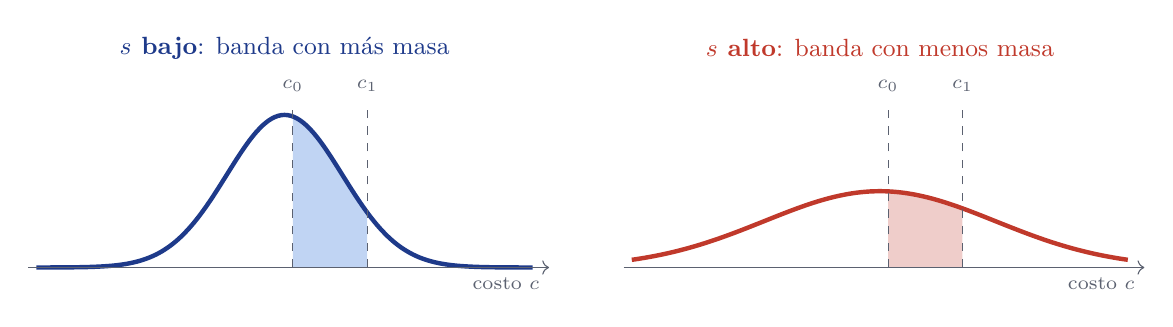
\begin{tikzpicture}[xscale=1.05,yscale=3.4]
    % s bajo
    \begin{scope}
      \fill[upaccent!30,domain=0.1:1.0,smooth,variable=\x] (0.1,0) -- plot (\x,{exp(-(\x)^2/(2*0.49))/(0.7*2.5066)}) -- (1.0,0) -- cycle;
      \draw[line width=1.6pt,upblue,domain=-3:3,smooth,samples=80] plot (\x,{exp(-(\x)^2/(2*0.49))/(0.7*2.5066)});
      \draw[->,upgray] (-3.1,0) -- (3.2,0) node[below left,font=\scriptsize]{costo $c$};
      \draw[dashed,upgray] (0.1,0) -- (0.1,0.62) node[above,font=\scriptsize]{$c_0$};
      \draw[dashed,upgray] (1.0,0) -- (1.0,0.62) node[above,font=\scriptsize]{$c_1$};
      \node[font=\small,upblue] at (0,0.82) {\textbf{$s$ bajo}: banda con más masa};
    \end{scope}
    % s alto
    \begin{scope}[xshift=7.2cm]
      \fill[upred!25,domain=0.1:1.0,smooth,variable=\x] (0.1,0) -- plot (\x,{exp(-(\x)^2/(2*1.96))/(1.4*2.5066)}) -- (1.0,0) -- cycle;
      \draw[line width=1.6pt,upred,domain=-3:3,smooth,samples=80] plot (\x,{exp(-(\x)^2/(2*1.96))/(1.4*2.5066)});
      \draw[->,upgray] (-3.1,0) -- (3.2,0) node[below left,font=\scriptsize]{costo $c$};
      \draw[dashed,upgray] (0.1,0) -- (0.1,0.62) node[above,font=\scriptsize]{$c_0$};
      \draw[dashed,upgray] (1.0,0) -- (1.0,0.62) node[above,font=\scriptsize]{$c_1$};
      \node[font=\small,upred] at (0,0.82) {\textbf{$s$ alto}: banda con menos masa};
    \end{scope}
  \end{tikzpicture}
  \end{center}
  \vspace{-0.1cm}
  {\footnotesize Cuando la banda contiene el centro de la distribución, más dispersión \textbf{saca} votantes marginales de ella. Si la banda estuviera en una cola, el efecto se invertiría.\par}
\end{frame}

% ===== 13. Por qué no está resuelto (1:30) =====
\begin{frame}{Por qué este resultado no está resuelto}
  \footnotesize
  \renewcommand{\arraystretch}{1.4}
  \begin{tabularx}{\textwidth}{@{}L{3.6cm}YY@{}}
    \toprule
    \textbf{Trabajo} & \textbf{Qué hace} & \textbf{Qué le falta} \\
    \midrule
    Panagopoulos (2008) & Sanción en el cálculo del voto & Perfil por edad y agregación: no dice qué mide una brecha entre intervalos \\
    Gonzales, León-Ciliotta y Martínez (2022) & Exención de los 70 con edades simples (${\sim}20$ pp entre 69 y 72 años) y reforma de multas de 2006 & Su estimando es el lado derecho de (i), no $\Delta$; sin curvatura en la sanción \\
    J.\,H.\ Fowler (2006) & Hábito de votar & Sin sanciones \\
    Jaitman (2013); Cepaluni y Hidalgo (2016) & RDD en umbrales de edad, Argentina y Brasil & Forma reducida, sin modelo \\
    \rowcolor{uplight}\textbf{Esta propuesta} & \textbf{Modelo de $\tau^{70}$ y de la brecha agregada} & \textbf{Resultados (a)-(d) y (i)-(iv)} \\
    \bottomrule
  \end{tabularx}
  \vspace{0.1cm}
  {\scriptsize\color{upgray} Dónde busqué: versión publicada de Gonzales et al.\ (\textit{AEJ: Applied}, 2022), su documento de trabajo (CEPR DP 13898) y sus diapositivas de la AEA 2020. Encuentran que eliminar toda la multa tiene menos de 1/5 del efecto de la exención: la sanción relevante no es solo $qF$.\par}
\end{frame}

% ===== 15. Límites y paper final (1:00) =====
\begin{frame}{Límites y plan para el paper final}
  \renewcommand{\itemgap}{0.7em}
  \begin{columns}[T]
    \begin{column}{0.48\textwidth}
      \textbf{\color{upred}Límites}
      \small
      \begin{itemize}
        \item La heterogeneidad persistente y los shocks transitorios se suman en $c$: (iv) no los distingue.
        \item Si el hábito de 70+ se deprecia, (i) se refuerza, pero no se separa del envejecimiento con cortes transversales.
        \item Que $B$ no crezca desde los 60 es un supuesto del modelo, no un resultado.
      \end{itemize}
    \end{column}
    \begin{column}{0.48\textwidth}
      \textbf{\color{upblue}Paper final}
      \small
      \begin{itemize}
        \item \textbf{Probar} (a)-(d) y (i)-(iv) completas; condiciones bajo las cuales (i) es estricta y una condición más general para (iv).
        \item \textbf{Simular} en \texttt{code/verify.py}: SymPy para las derivadas, Monte Carlo sobre perfiles $B(a)$ no crecientes; el contraejemplo de (iv) como caso que debe fallar.
        \item \textbf{Lean}: edades discretas (sumas finitas). (a), (i), (ii) son análisis real elemental; (d), (iv) exigen derivar $F((x-\mu)/s)$ en $s$.
      \end{itemize}
    \end{column}
  \end{columns}
\end{frame}

% ===== 15b. Riesgos (1:00) =====
\begin{frame}{El paso con más riesgo: (d) y (iv) frente a los datos}
  \begin{block}{La hipótesis de (d) puede fallar en 3 de las 5 elecciones del gráfico}
    \small Como $B$ no crece con la edad, $P_0(70)\ \ge\ \mathbb E_{a\ge 70}\big[P_0(a)\big]$. En la ONPE el grupo 70+ supera el 50\% en \textbf{2006, 2011 y 2016}: ahí $P_0(70)>50\%$, la condición de (d) \alert{falla} y el signo de $\partial\tau^{70}/\partial s$ puede invertirse.
  \end{block}
  \vspace{0.1cm}
  \small
  \renewcommand{\itemgap}{0.5em}
  \begin{itemize}
    \item Si es así, (iv) queda como resultado condicional: el signo depende de dónde cae la banda.
    \item $G$ igual a toda edad es fuerte: el costo de votar sube con la edad; si $G$ depende de $a$, (i) necesita dominancia estocástica.
    \item Supervivencia selectiva de los muy mayores puede violar la monotonía de $B$ en el corte transversal; el padrón con fallecidos no depurados infla $\Delta$.
  \end{itemize}
\end{frame}

% ===== 16. Cierre =====
{
\setbeamertemplate{footline}{}
\begin{frame}
  \begin{center}
    \vspace{0.8cm}
    {\color{upblue}\Huge\bfseries Gracias}\\[0.5cm]
    {\large Comentarios y preguntas}\\[0.9cm]
    {\small Manuel Arriola Montenegro}\\[0.1cm]
    {\small\color{upaccent}\texttt{github.com/Arriola123456/ai-project}}\\[0.25cm]
    
\includegraphics[height=1cm]{logo.png}
  \end{center}
\end{frame}
}

\end{document}
